%%% PG DAY FR 2013, Nantes, 13 Juin
%%%
%%% Les prochains développements à suivre pour le Big Data sans soucis sous
%%% PostgreSQL.
%%%
%%% PostgreSQL est le système de gestion de bases de données dont la
%%% progression est la plus rapide et la mieux soutenue. Il reste beaucoup à
%%% apporter au projet afin de permettre d'exploiter sereinement quelques
%%% Peta Octets de données. Cette présentation entend faire un tour des
%%% projets les plus significatifs dans cette direction, qu'ils soient en
%%% cours de conception, de réalisation ou bien encore embryonnaires.

\documentclass{beamer}

\usepackage{beamerthemesplit}
\usepackage[utf8]{inputenc}
%% \usetheme{AnnArbor}
\usetheme{Boadilla}
%% \usetheme{Pittsburgh}
%% \usecolortheme{beaver}
\beamertemplatetransparentcovered

\title{vers le PetaByte}
\subtitle{avec PostgreSQL}
\author{Dimitri Fontaine \texttt{dimitri@2ndQuadrant.fr}}
\date{13 Juin 2013}
\logo{
\includegraphics[height=0.4cm]{2ndQuadrant-cross.png}}

\begin{document}

\frame{\titlepage}

\section{Introduction}

\begin{frame}[fragile]
  \frametitle{Dimitri Fontaine}

  \begin{center}
    \textbf{2ndQuadrant France}
    \linebreak
    PostgreSQL Major Contributor
  \end{center}
  \linebreak

\begin{columns}[c]
\column{.75\textwidth} 

  \begin{itemize}
   \item \texttt{pgloader}, \texttt{prefix}, \texttt{skytools}, \texttt{debian}, …
   \item \texttt{\textbf{CREATE EXTENSION}}
   \item \texttt{\textbf{CREATE EVENT TRIGGER}}
   \item \textit{Bi-Directional Réplication}
   \item \textit{Partitionnement}
  \end{itemize}  

\column{.25\textwidth}
\begin{center}
  
\includegraphics[height=5em]{bulle-blue-icon.png}
\end{center}
\end{columns}
\end{frame}

\begin{frame}
  \frametitle{C'est quoi un \textit{PetaByte}?}

  \center{\textbf{Beaucoup} de données}
  \vfill

\begin{columns}[c]
\column{.55\textwidth} 
  
  \center{\texttt{1 PB =}}
  \vfill

  \begin{itemize}
  \item \texttt{1 024} \textbf{TB}
  \item \texttt{1 048 576} \textbf{GB}
  \item \texttt{1 073 741 824} \textbf{MB}
  \item \texttt{1 099 511 627 776} \textbf{KB}
  \item \texttt{1 125 899 906 842 624} \textbf{Bytes}
  \end{itemize}

\column{.45\textwidth}
\begin{center}
  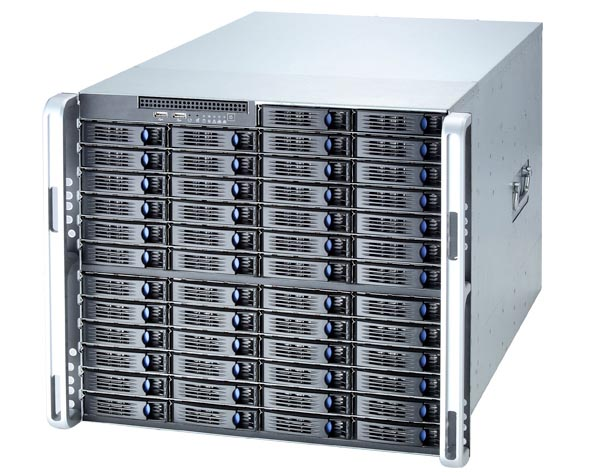
\includegraphics[height=13em]{119tera.jpg}
\end{center}
\end{columns}
\end{frame}
\end{frame}

\begin{frame}[fragile]
\begin{center}
  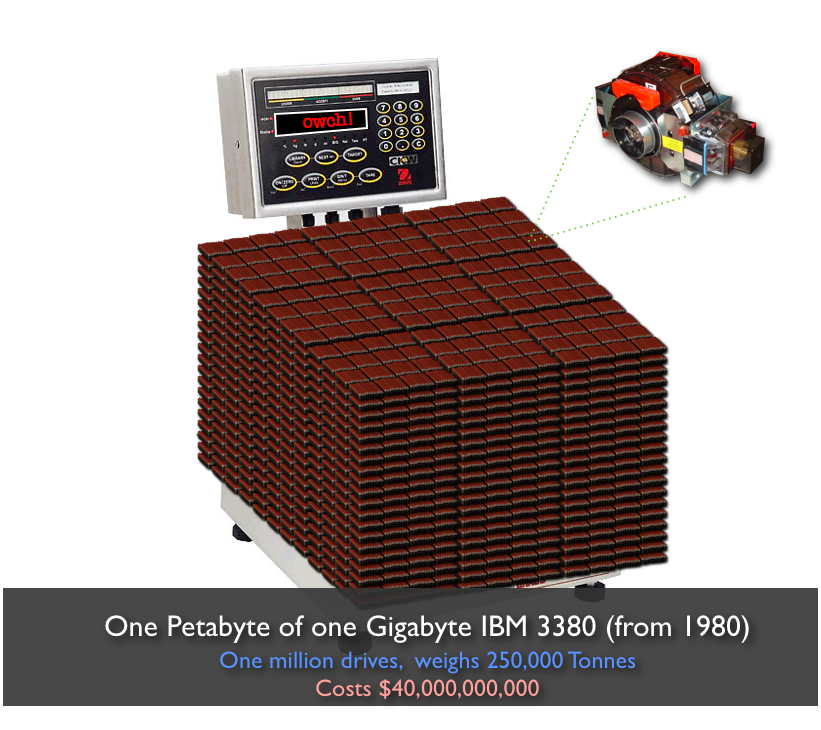
\includegraphics[height=22em]{1pbibm1.png}
\end{center}
\end{frame}

\begin{frame}[fragile]
\begin{center}
  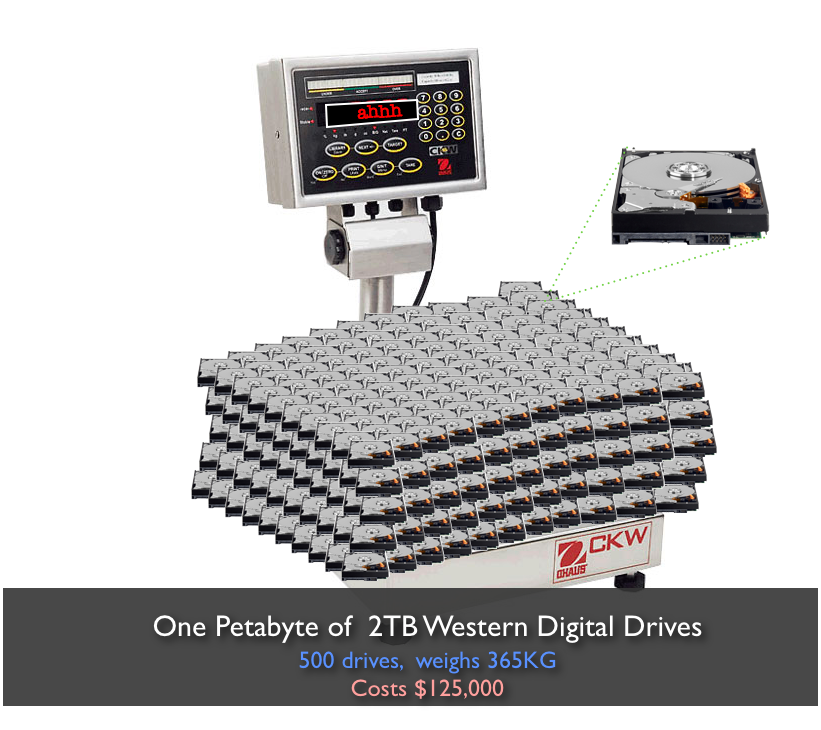
\includegraphics[height=22em]{1pbwd.png}
\end{center}
\end{frame}

\begin{frame}[fragile]
\begin{center}
  \center{\Huge Big Data ?}
  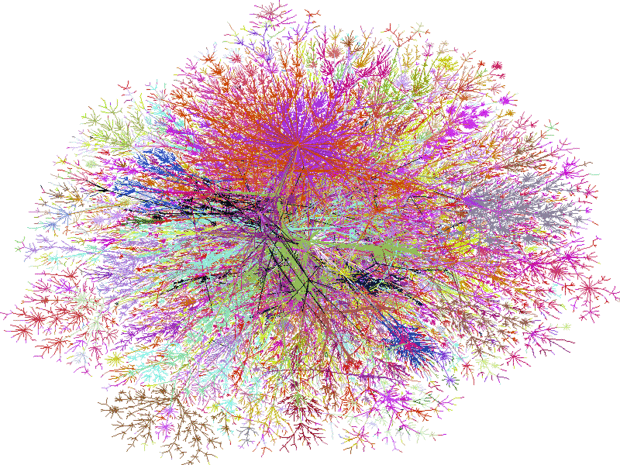
\includegraphics[height=18em]{bigdata.png}
\end{center}
\end{frame}

\begin{frame}[fragile]
\begin{center}
  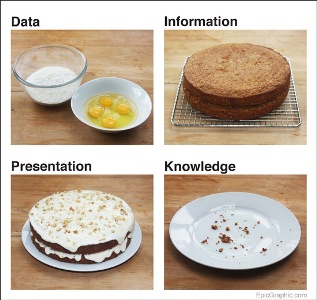
\includegraphics[height=18em]{OCDQ_cake1.jpg}
\end{center}
\end{frame}

\begin{frame}[fragile]
\begin{center}
  \frametitle{Maintenance et Volumes des bases de données}

  \center{\textit{The Horizontal Struggle}}

  \begin{itemize}
  \item \texttt{0.1 GB} schema, backup : seconds
  \item \texttt{1 GB} schema : seconds, backup : minutes (a few)
  \item \texttt{10 GB} schema : depends, backup : minutes (many)
  \item \texttt{100 GB} schema, backup : hours
  \item \texttt{1 TB} schema : difficult, backup : days
  \end{itemize}
\end{center}
\end{frame}

\begin{frame}[fragile]
\begin{center}
  \frametitle{VACUUM, AUTO VACUUM}
  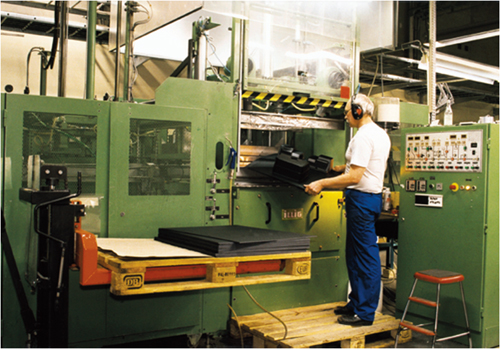
\includegraphics[height=20em]{VacuumForming.jpg}
\end{center}
\end{frame}

\begin{frame}[fragile]
\begin{center}
  \frametitle{INDEXES}
  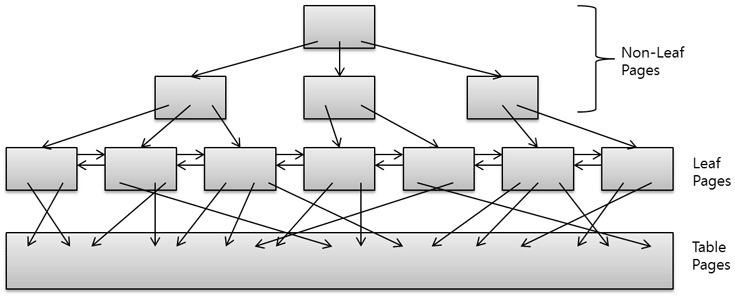
\includegraphics[height=12em]{b+tree-structure.png}
\end{center}
\end{frame}

\begin{frame}[fragile]
\begin{center}
  \frametitle{CHECKPOINT}
  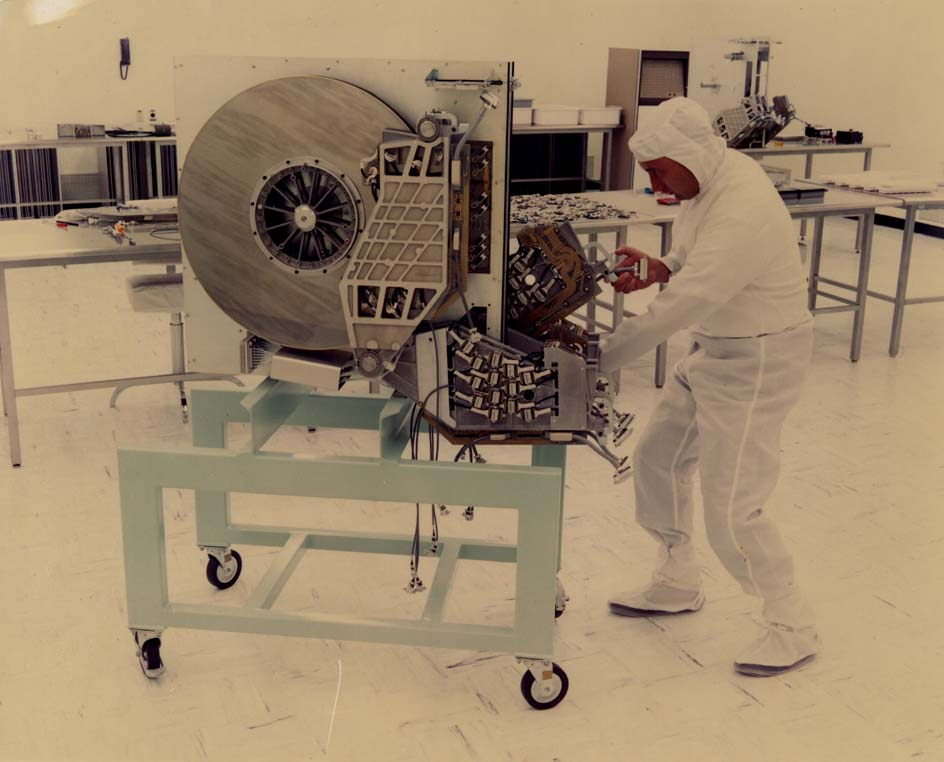
\includegraphics[height=20em]{new_hard_drive.jpg}
\end{center}
\end{frame}

\begin{frame}[fragile]
\begin{center}
  \frametitle{Sauvegardes, \texttt{pg\_dump}, \texttt{basebackup}}

  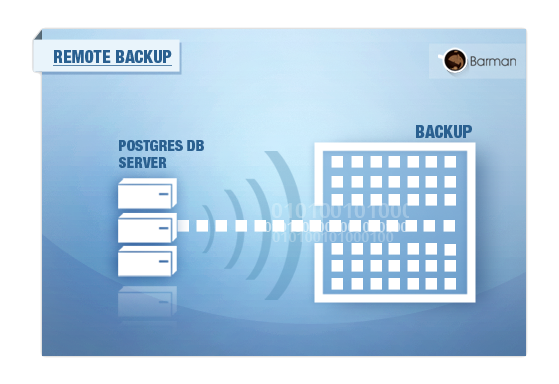
\includegraphics[height=20em]{barman.png}
\end{center}
\end{frame}

\begin{frame}[fragile]
\begin{center}
  \frametitle{Archivage, \texttt{PITR}}

  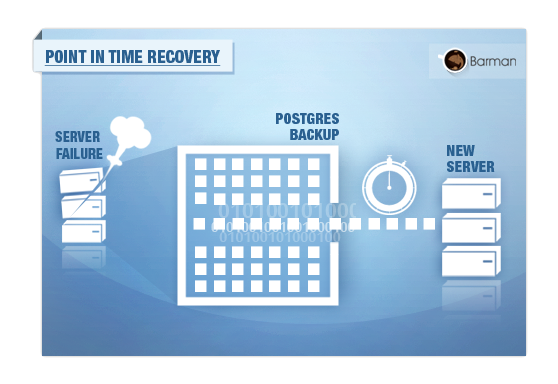
\includegraphics[height=20em]{barman-pitr.png}
\end{center}
\end{frame}

\begin{frame}[fragile]
\begin{center}
  \frametitle{Replication}

  
\includegraphics[height=20em]{Regions-Zones.png}
\end{center}
\end{frame}

\begin{frame}[fragile]
  \frametitle{Développements en cours}

  \begin{center}
  
\includegraphics[height=5em]{babysteps-300x300.jpg}
  \end{center}
  \vfill

\begin{columns}[c]
\column{.5\textwidth} 
  \begin{itemize}
  \item \texttt{CHECKSUM}
  \item \texttt{COPY FREEZE}
  \item \texttt{work\_mem}
  \end{itemize}

\column{.5\textwidth}
  \begin{itemize}
  \item \texttt{REINDEX CONCURRENTLY}
  \item \texttt{VACUUM FREEZE, XID EPOCH}
  \item \texttt{work\_mem > 1 GB}
  \end{itemize}
\end{columns}
\end{frame}

\begin{frame}[fragile]
\begin{center}
  \frametitle{Architectures distribuées}

  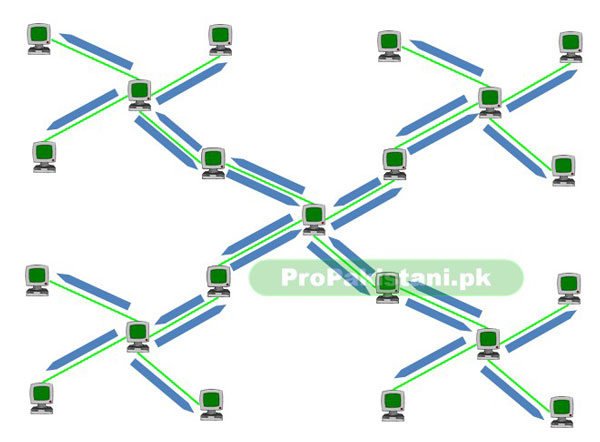
\includegraphics[height=20em]{p2p.jpg}
\end{center}
\end{frame}

\section{Conclusion}

\begin{frame}[fragile]
  \frametitle{Outils pour Architectures Distribuées}

  \begin{center}
    \textbf{Bi Directional Replication}
    \vfill
    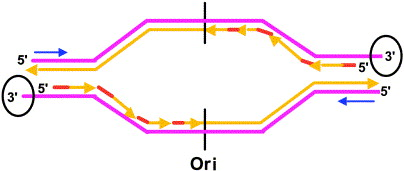
\includegraphics[height=12em]{bdr.jpg}
  \end{center}

\begin{columns}[c]
\column{.6\textwidth} 
  \begin{itemize}
    \item \textit{Read/Write} Foreign Data Wrappers
  \end{itemize}
\column{.4\textwidth}
  \begin{itemize}
    \item PL/Proxy
  \end{itemize}
\end{columns}
\end{frame}

\begin{frame}[fragile]
  \frametitle{Conclusion}
  \begin{center}
    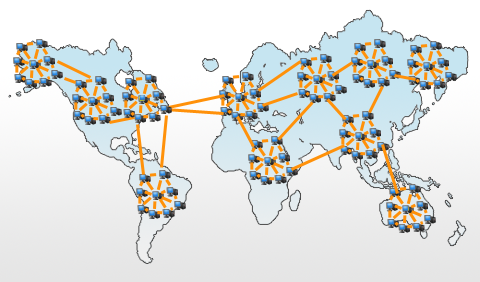
\includegraphics[height=14em]{p2p-world.png}
  \end{center}
\end{frame}

\end{document}
